\section{Theorie}
\label{sec:Theorie}

Ziel dieses Versuches ist die Bestätigung der Quantennatur der Elektronenhüllen von 
Atomen.\\

Zu diesem Zweck werden beschleunigte Elektronen zur Anregung von Atomen 
im Quecksilberdampf genutzt. Bei kleinen Energien kommt es dabei zunächst zu 
elastischen Stößen der Elektronen mit den Hg-Atomen, bei denen noch keine Anregung
zustande kommt, allein die Elektronenbewegungsrichtung wird dabei aufgrund des ungleichen 
Masseverhältnisses $\frac{m_e}{M} = 1836,201$ beeinflusst. Die Hg-Atommasse $M >> m_e$ ist 
sehr viel größer als die Elektronenmasse $m_e$, daher
geben die Elektronen hier nur den vernachlässigbar kleinen Energiebetrag

\begin{equation}
    \symup{\Delta} E = \frac{4 m_e M}{(m_e + M)^2} \cdot E
\end{equation}

an die Hg-Atome ab. $E$ beschreibt dabei die kinetische Energie der Elektronen.\\

Erst ab einer bestimmten Energiehürde stoßen die Elektronen der Geschwindigkeit
$v_\text{vor}$ und der Masse $m_e$ mit den Hg-Atomen, die vereinfacht nach dem Bohrschen Atommodell betrachtet werden,
unelastisch zusammen, regen die Atome in den ersten diskreten angeregten Zustand an und geben dabei
die Energiedifferenz

\begin{equation}
    E_1 - E_0 = \frac{m_e \cdot v_\text{vor}^2}{2} - \frac{m_e \cdot v_\text{nach}^2}{2}
\end{equation}
 
ab. Im Detail wird jeweils eins der $2$ s-Elektronen der Valenzschale auf das Energieniveau der nächsthöheren Schale
gehoben. Nach dem Stoß besitzen die Stoßlektronen nur noch die Geschwindigkeit $v_\text{nach}$ und die Energie
$E - (E_1 - E_0)$.
Die verbliebene Elektronenenergie soll dabei nach der Gegenfeldmethode gemessen werden.

Die Hg-Atome emittieren nach der Relaxationszeit die überflüssige Anregungsenergie wieder
in Form eines Photos mit der Energie 

\begin{equation}
    h \nu = E_1 - E_0 \; .
\end{equation}

Dementsprechend ist theoretisch die in Abbildung \ref{fig:bild2} dargestellte Strom-Spannungskurve zu messen.

\begin{figure} [H]
    \centering
    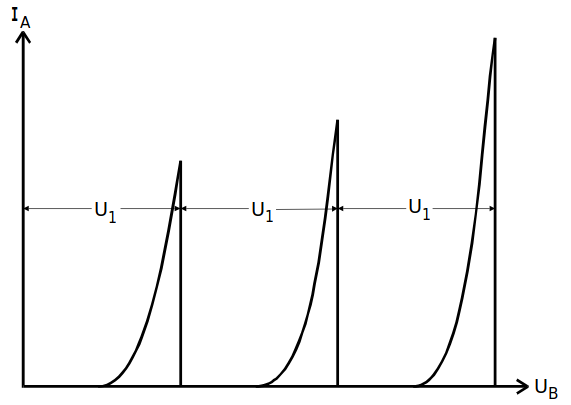
\includegraphics[scale=0.4]{content/bild2.png}
    \caption{Idealisierte Strom-Spannungskurve des Franck-Hertz-Versuches [1]}
    \label{fig:bild2}
  \end{figure}

  Es ist zu erkennen dass der Auffängerstrom $I_\text{A}$ bei steigender Beschleunigungsspannung $U_\text{B}$
  solange steigt, bis $E$ für unelastische Stöße der Elektronen mit den Hg-Atomen ausreicht. Danach
  fällt $I_\text{A}$ plötzlich ab. Bei weiterer Steigerung von $U_\text{B}$ steigt auch $I_\text{A}$,
  bis $E$ dann ausreicht, um jeweils zwei unelastische Stöße der Elektronen mit den Hg-Atomen zuzulassen.
  Dies wiederholt sich bei steigender $U_\text{B}$ bis hin zu mehreren Anregungen.
  Die Spannungsdifferenzen zwischen den Strommaxima betragen dabei

  \begin{equation}
      \symup{\Delta}U = \frac{E_1 - E_0}{e_0} \; .
  \end{equation}

Außerdem können die Hg-Atome durch Elektronenstöße ionisiert werden.
Die dazu nötige Ionisationsenergie kann auch bestimmt werden. 

%_________________________________________________________________________________

\subsection{Einflüsse auf den Verlauf der Franck-Hertz-Kurve}

\subsubsection{Einfluss des Kontaktpotentials}

Aufgrund verschiedener Austrittsarbeiten $\phi_\text{G}$ und $\phi_\text{B}$ der Glühkathode 
und Beschleunigungsanode kommt es zu einem in Abbildung \ref{fig:bild3} dargestelltem Potentialgefälle,

\begin{figure} [H]
    \centering
    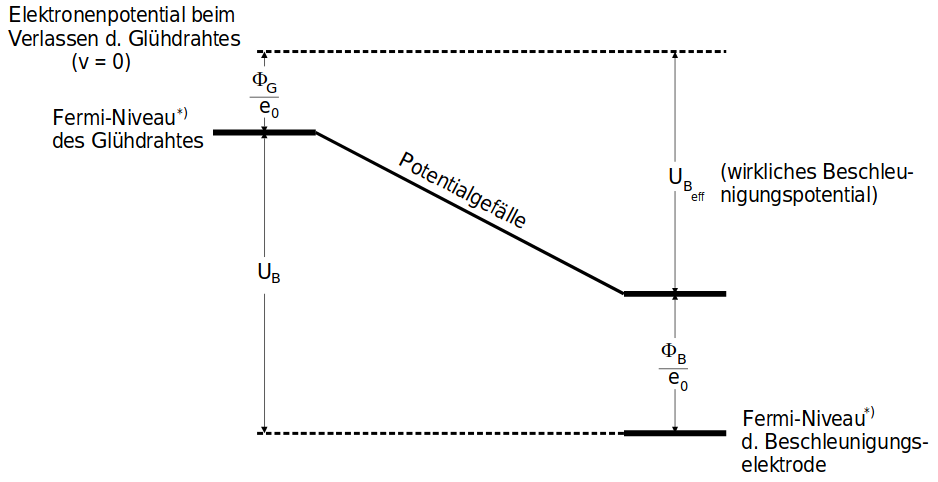
\includegraphics[scale=0.4]{content/bild3.png}
    \caption{Das aus den verschiedenen Austrittsarbeiten der Elektroden resultierende Potentialgefälle [1]}
    \label{fig:bild3}
  \end{figure}

wodurch die effektive Beschleunigungsspannung nur noch

\begin{equation}
    U_\text{B,eff} = U_\text{B} - \frac{\phi_\text{B} - \phi_\text{G}}{e_0}
\end{equation}

beträgt und die Franck-Hertz-Kurve um $\frac{\phi_\text{B} - \phi_\text{G}}{e_0}$ verschoben ist.

\subsubsection{Einfluss der Fermi-Dirac-Verteilung}

Da die Elektronen schon in der Glühkathode keinen diskreten Energiewert besitzen, sondern
ihre Energien verschiedene Werte der kontinuierlichen Fermi-Dirac-Verteilung annehmen,
sind auch ihre kinetischen Energien in der Vakuumkammer kontinuierlich verteilt.
Somit fällt die Franck-Hertz-Kurve nicht bei einem bestimmten Betrag von $U_\text{B}$ plötzlich
unstetig ab, sondern nähert sich stetig einem Stromminimum.

\subsubsection{Der Einfluss des Dampfdruckes}

Der Franck-Hertz-Versuch erzielt die erwarteten Messwerte bei einer bestimmten Dampfdichte am besten.
Ist die Dampfdichte bspw. sehr klein, so kann es auch bei sehr großer $U_\text{B}$ nur vereinzelt
zu Anregungen kommen, da die Stoßwahrscheinlichkeit sehr klein ist. Bei sehr hohen Dampfdichten 
spielt der Energieverlust durch elastische Stöße eine immer größere Rolle.


%____________________________________________________________________________________________

\subsection{Der Versuchsaufbau und die Gegenfeldmethode}

Der Versuchsaufbau ist in Abbildung \ref{fig:bild1} dargestellt.

\begin{figure} [H]
    \centering
    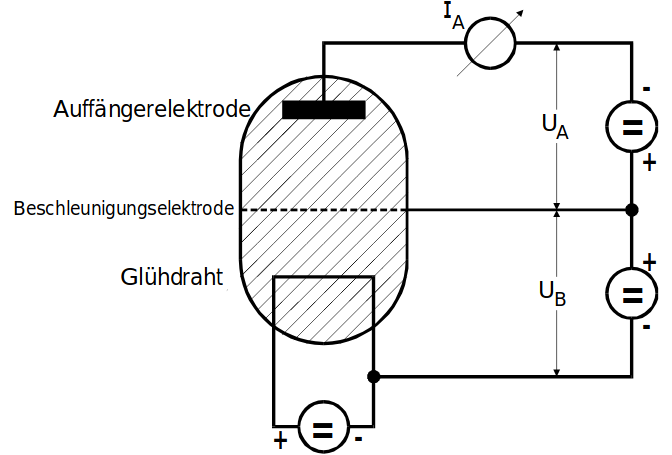
\includegraphics[scale=0.4]{content/bild1.png}
    \caption{Versuchsaufbau des Franck-Hertz-Versuchs [1]}
    \label{fig:bild1}
  \end{figure}

In einem evakuierten Gefäß, in dem ein Quecksilbertropfen verdampft sind
eine Glühkathode, Bescheunigungsgitteranode und eine Auffängerelektrode eingefasst.

Die aus der Glühkathode emittierten Elektroden werden durch das von der
Beschleunigungsspannung $U_\text{B}$ erzeugte E-Feld zur Gitteranode hin
beschleunigt.

Die kinetische Elektrodenenergie kann als

\begin{equation}
    \frac{m_e \cdot v_\text{vor}^2}{2} = e_0 \cdot U_\text{B}
\end{equation}

bestimmt werden.

Danach werden die Elektronen im durch die Bremsspannung $U_\text{A}$ erzeugten
Gegenfeld gebremst. 

Es können nur die Elektronen das Gegenfeld überwinden, für die deren kinetische
Energie entlang des Feldes die Ungleichung

\begin{equation}
    \frac{m_e \cdot v_\text{E}}{2} \geq e_0 \cdot U_\text{A}
\end{equation}

erfüllt.
Es wird der Auffängerstrom $I_\text{A}$ der nach den Stößen dennoch an der Auffängerelektrode ankommenden
Elektronen gemessen.

Außerdem lässt sich die Quecksilberdampfdichte durch Temperaturänderung regeln.

